\documentclass{llncs}
\usepackage{times}
\usepackage[T1]{fontenc}

% Comentar para not MAC Users
%\usepackage[applemac]{inputenc}

\usepackage{a4}
%\usepackage[margin=3cm,nohead]{geometry}
\usepackage{epstopdf}
\usepackage{indentfirst}
\usepackage{graphicx}
\graphicspath{{Capturas-Ecra/}}
\usepackage{float}
\usepackage{fancyvrb}
\usepackage{amsmath}
\usepackage{array}
\usepackage{courier} %% Sets font for listing as Courier.
\usepackage{listings, xcolor}
\lstset{
tabsize = 4, %% Sets tab space width.
showstringspaces = false, %% Prevents space marking in strings, string is defined as the text that is generally printed directly to the console.
numbers = left, %% Displays line numbers on the left.
commentstyle = \color{green}, %% Sets comment color.
keywordstyle = \color{blue}, %% Sets  keyword color.
stringstyle = \color{red}, %% Sets  string color.
rulecolor = \color{black}, %% Sets frame color to avoid being affected by text color.
basicstyle = \small \ttfamily , %% Sets listing font and size.
breaklines = true, %% Enables line breaking.
numberstyle = \tiny,
}
%\renewcommand{\baselinestretch}{1.5}

\setcounter{secnumdepth}{4} % how many sectioning levels to assign numbers to
\setcounter{tocdepth}{4}

\begin{document}
\mainmatter
\title{TP2 - Serviço de transferência rápida e fiável de dados sobre UDP}

\titlerunning{TP2 - Serviço de transferência rápida e fiável de dados sobre UDP}

\author{Diogo Braga \and João Silva}

\authorrunning{Diogo Braga \and João Silva}

\institute{
University of Minho, Department of  Informatics, 4710-057 Braga, Portugal\\
e-mail: \{a82547,a82005\}@alunos.uminho.pt\\
PL2, Grupo 6
}

\date{}
\bibliographystyle{splncs}

\maketitle

\section{Introdução}

Neste relatório são apresentadas as informações e decisões tomadas relativamente ao projeto no qual o objetivo era criar um serviço de transferência fiável de dados sobre o protocolo UDP. São abordados temas como, por exemplo, o formato das mensagens PDU, as interações entre os end-systems, a arquitetura criada para a implementação e o controlo de fluxo e de congestão nas transferências de dados. Estão também presentes testes e resultados, assim como uma secção de conclusões.


\section{Especificação do protocolo}




\subsection{Formato das mensagens protolocares (PDU)}

O formato escolhido engloba aspetos que segmentos UDP por norma não incluem. Escolhemos tal abordagem para conseguir implementar uma comunicação fiável por cima dum transporte UDP. O formato escolhido é apresentado abaixo.

\begin{lstlisting}[language = Java , frame = trBL , firstnumber = last , escapeinside={(*@}{@*)}]
	private int sequence_number;
	private int ack_number;
	private String options;
	private boolean syn;
	private boolean fin;
	private boolean ack;
	private boolean psh;
	private int receiveWindow;
	private long checksum;
	private byte[] data;
\end{lstlisting}

Em cada \textbf{PDU} enviado estes parâmetros vão preenchidos com informação relevante para que se mantenha uma comunicação fiável, e se consiga manter um estado da comunicação. Desta forma asseguramos uma implementação dum protocolo orientado à comunicação tendo por base \textbf{UDP}.

Os campos \textbf{sequence\_number} e \textbf{ack\_number} servem para que se mantenha uma sequência no transferência dum ficheiro, e poder saber sempre se segmentos foram perdidos ou chegaram fora de ordem por exemplo.

Os campos \textbf{syn}, \textbf{fin}, \textbf{ack} e \textbf{psh} servem para identificar que tipo de segmento se trata, tendo em consideração o cabeçalho do \textbf{TCP} que contempla estes campos.

O campo \textbf{options} é usado para que sejam transferidas informações adicionais sobre a transferência dum ficheiro. É usado, por exemplo, no início da conexão para enviar o número de segmentos que o ficheiro contempla.

Usamos o campo \textbf{receiveWindow} para que trocar informação sobre o possível espaço em buffer para receber datagramas. Server para controlar o fluxo da comunicação.

O campo \textbf{data} leva todos os dados a transferir relativos ao ficheiro. Este campo tem no máximo \textbf{1024} bytes (MSS), por forma a otimizar o processo de envio tendo os segmentos relativamente curtos, para que a probabilidade de serem partidos em camadas inferiores seja reduzida.

Por último, o campo \textbf{checksum} leva um inteiro (long), relativo ao cálculo do checksum o do campo \textbf{data}.


\subsection{Interações}

\subsubsection{Início de Conexão}

\hspace{20.0cm}

Para ocorrer uma transferência de dados entre dois end-systems é necessário que exista inicialmente um estabelecimento de conexão. Quem pretende iniciar uma conexão envia um \textbf{syn} para o destino, na esperança de receber um \textbf{synack} do servidor ao qual se liga. Seguidamente o cliente envia também um \textbf{ack} a confirmar o estabelecimento da conexão. Desta forma, com este processo tornamos a comunicação orientada à conexão, e portanto, mais controlada.

\subsubsection{Transferência de Ficheiro}

\hspace{20.0cm}

Depois de estabelecida a conexão, é realizado o envio dos dados por parte do servidor tendo em conta os parâmetros estabelecidos, como por exemplo a janela de receção de dados e o MSS. Nesta fase existe também muita interação entre os dois end-systems, pois após a tentativa de envio do servidor, o cliente têm que enviar um ack para confirmar a receção dos dados. Existe a possibilidade deste não chegar ao destino devido a congestionamentos na camada de Rede, de tal forma que nesta fase existem também retransmissões, caso necessário.

\subsubsection{Fim de Conexão}

\hspace{20.0cm}

Devido a estarmos perante uma comunicação orientada à conexão, é necessário que, depois da transferência dos dados, esta seja terminada. No nosso modelo tal acontece da seguinte forma: servidor enviar \textbf{fin} para o cliente a sinalizar que terminou a transferência dos dados; cliente responde com \textbf{finack} para sinalizar receção do fin; servidor envia \textbf{ack} para sinalizar que recebeu a confirmação do fecho da conexão do lado do cliente.



\section{Implementação}

Nesta secção optamos por fazer uma abordagem Top-Down da nossa implementação, começando pela interface com o utilizador até à classe responsável por receber e enviar datagramas pelo socket. Utilizamos a linguagem \textbf{Java} para tal tarefa.


\subsection{Interface}

A primeira fase da transferência inicia com uma interação com o software criado, tanto por parte de quem disponibiliza o ficheiro para upload (servidor), como por parte de quem tenciona descarregá-lo (cliente).

Tal interação é especificada no ficheiro \textbf{TransfereCCcmd.java}. Dependendo do que é pretendido fazer invocam-se diferentes comandos, exemplificados a seguir.

\begin{verbatim}
	>  java TransfereCCcmd -put Teste.txt
\end{verbatim}

Neste caso quem invoca o comando está a disponibilizar o ficheiro \textit{Teste.txt} para possível upload por parte de vários clientes. O utilizador terá de terminar o processo quando desejar uma vez que funciona como servidor para vários clientes e não se cinge só a uma transferência.

\begin{verbatim}
	>  java TransfereCCcmd -get Saida1.txt 10.1.1.1
\end{verbatim}

Neste caso quem invoca o comando tenciona fazer download do ficheiro que está (ou não) a ser disponibilizado por \textbf{10.1.1.1}. O ficheiro que será descarregado terá o nome \textit{Saida1.txt}.

\begin{verbatim}
	>  java TransfereCCcmd -help
\end{verbatim}

Neste caso o utilizador consulta a forma de utilização do software.


\subsection{Gestor de Transferências}

Dependendo de como o utilizador se identifica na interface (Upload ou Download) é criada uma Thread correspondente à classe \textbf{TransfereCC} que atua de diferente forma caso esteja a ser feito um Upload ou um Download. Em ambos os casos a primeira coisa a ser feita pelo \textbf{TransfereCC} é a criação duma Thread correspondente à classe \textbf{AgenteUDP} que reside no ficheiro \textbf{AgenteUDP.java}. Esta classe será abordada numa secção subsequente.

O \textbf{TransfereCC} tem um função que passa por receber datagramas provenientes do \textbf{AgenteUDP}, desserializar bytes recebidos transformando-os num \textbf{PDU}. Testa o \textbf{checksum} do segmento, sendo esta uma fase crucial pois em caso de erro descarta o \textbf{PDU} recebido, em situação afirmativa entrega-lo à Thread responsável pelo \textbf{IP} de origem (caso do Upload).


\subsubsection{Download}

\hspace{20.0cm}

Em caso de Download é criada uma única Thread que irá tratar de todo este processo correspondente à classe \textbf{ThreadDownload} que se encontra no ficheiro \textbf{ThreadDownload.java}.

Esta Thread tem 3 principais estados que são o início de conexão, a transferência de dados relativos ao ficheiro, e o fim da conexão.

Durante o processo de transferência de dados relativos ao ficheiro esta Thread recebe e confirma todos os PDUs recebidos do servidor atuando com um mecanismo de \textbf{Selective Repeat}. Em caso de receber PDUs com um número de sequência maior do que aquele que estava à espera não envia para trás ACKs negativos mas sim um PDU com o número de sequência igual ao número de sequência que estava à espera, atuando desta forma igual ao \textbf{TCP}. Recebendo o segmento que estava à espera envia um possível \textbf{ACK cumulativo} confirmando todos os segmentos com números de sequência superiores que recebeu enquanto aguardava o segmento perdido/descartado.

Antes de todo este processo de transferência de dados iniciar é inicializada uma Thread correspondente à classe \textbf{ConsoleProgressBar}, que se encontra no ficheiro \textbf{ConsoleProgressBar.java} cuja única função é receber o progresso da transferência por parte da \textbf{ThreadDownload} e imprimir de forma muito elucidativa no ecrã o progresso da transferência dando uma perspetiva ao utilizador se ainda falta muito para a transferência terminar ou não.

No final junta tudo o que recebeu e cria um novo ficheiro com o nome passado como parâmetro inicialmente.


\subsubsection{Upload}

\hspace{20.0cm}

Em caso de Upload o processo é um pouco mais complexo que em caso de Download pois vai requerer um maior esforço por parte do \textbf{TransfereCC}, pois vai ter de manter um \textbf{Map} associando um \textbf{IP} à Thread que trata do mesmo e tendo que entregar datagramas a estas Threads.

Quando o \textbf{TransfereCC} recebe um datagrama cujo IP não está mapeado na sua estrutura, trata de criar uma Thread correspondente à classe \textbf{ThreadUpload}, que se encontra no ficheiro \textbf{ThreadUpload.java} e associando-a ao IP correspondente na sua estrutura.

Tal como em caso de Download esta Thread tem 3 principais fases que são o início de conexão, a transferência de dados relativos ao ficheiro, e o fim da conexão.

Quando é feito uma comunicação fiável é necessário que se envie segmentos com os dados necessários para o destinatário mas ao mesmo tempo tem que se ir confirmando se estamos a receber confirmações dos dados enviados. Ora como seria incômodo e provavelmente não real após enviar um segmento esperar a sua confirmação, foi necessário a criação de uma Thread capaz de tratar apenas dos ACKs recebido sendo estes válidos ou duplicados. Tal encontra-se na classe \textbf{UploadReceiver}, no ficheiro \textbf{UploadReceiver.java}.

Em caso de surgirem ACKs duplicados esta nova Thread trata de reenviar de imediato para o destinatário o segmento em falta, continuando o seu processo normal após esta ação.

Enquanto esta Thread recebe segmentos para interpretá-los, a \textbf{ThreadUpload} encontra-se num ciclo de envio ordenado de segmentos, previamente separados pelo \textbf{TransfereCC}.

Após a Thread de receção receber o último segmento dá sinal numa variável de condição que permite avançar para o término de conexão. Após terminar a conexão é dito ao \textbf{TransfereCC} que a conexão acabou e que a Thread relativa àquele IP pode ser removida do Map.


\subsection{Estado}

Ligado a cada transferência tanto dum Download como dum Upload está um estado implícito associado a cada Thread. Tal estado corresponde à classe \textbf{Estado}, que se encontra no ficheiro \textbf{Estado.java}.

Este estado alberga todas as burocracias que não devem ser mantidas pelas Threads que tratam da transferência mas sim por uma classe mais especializada neste tipo de dados. O Estado contém:

\begin{lstlisting}[language = Java , frame = trBL , firstnumber = 1 , escapeinside={(*@}{@*)}]
    private TransferState estado;
    private int sequence_number;
    private int first_data_seq_number;
    private int ack_number;
    private int first_data_ack_number;
    private int mss;
    private int receiveWindow;
    private CongestionControlPhase cc_phase;
    private int dupAckCount;
    private int ssthresh;
    private float congestionWindow;
    private long timeout; // milissegundos
    private long estimatedRTT;
    private long devRTT;
    private int timeout_count;
\end{lstlisting}

É no estado que são mantidos mecanismos de sequenciação, dados pelos parâmetros \textbf{sequence\_number}, \textbf{first\_data\_seq\_number}, \textbf{ack\_number} e \textbf{first\_data\_ack\_number}. Estes valores são acedidos pelas Threads para preencherem corretamente os valores dos campos dos PDUs.

Existem um campo que mantém o tamanho do \textbf{MSS} que porventura é sempre fixo e igual a 1024.

Existe a variável \textbf{receiveWindow} que contém o valor da janela associada ao controlo de fluxo. Este valor para o fluxo foi calculado tendo em conta o buffer de receção que tinha um espaço de 66560 bytes que dividindo por um segmento de 1024 bytes e tirando 10 (por precaução) devido a possíveis segmentos de tamanho maior, resulta numa janela de \textbf{55}.

Existe ainda um conjunto de variáveis associado ao controlo de fluxo. São nomeadamente \textbf{cc\_phase}, que nos dá o estado da congestão, \textbf{dupAckCount} que conta o número de ACKs duplicados, \textbf{ssthresh} que representa o threshold e por último a \textbf{congestionWindow} que representa o valor inteiro da janela de congestão.

Ora o valor de janela passado às Threads para elas trabalharem baseia-se no mínimo da janela de fluxo e da janela de congestão.

O estado contém ainda variáveis que tratam de valores de timeouts. Elas são nomeadamente o \textbf{timeout} que representa o valor do timeout em milissegundos, o \textbf{estimatedRTT} que representa o valor estimado do RTT, o \textbf{devRTT} que representa o desvio em milissegundos que o RTT pode assinalar e o \textbf{timeout\_count}.

Inicialmente, antes de existir qualquer conexão o valor do timeout é de 3000 milissegundos (3 segundos),  após existir comunicação é retirado o RTT da primeira troca de PDUs e o valor do timeout passa a ser fixo mas com um valor mais aproximado da realidade. Ao fim de 3 tiemouts a conexão é desfeita e terminada.



\subsection{AgenteUDP}

O \textbf{AgenteUDP} é um Thread com a única função de receber Datagramas provenientes da rede, e enviar Datagramas para a rede. Existe apenas uma Thread deste género independentemente do número de conexões existentes.

Todas as Threads que estão encarregues de enviar PDUs para a rede contactam esta classe presente no ficheiro \textbf{AgenteUDP.java}. As comunicações são sempre feitas num socket cuja porta é \textbf{7777}.

Recebendo PDUs das várias Threads esta classe tem ainda a função de serializá-los, para ser possível criar datagramas e enviá-los para a rede.


\section{Funcionalidades Adicionais}

\subsection{Servidor Multithreaded}
No trabalho decidimos implementar servidores multithreaded, ou seja, servidores que disponibilizam um ficheiro no qual vários clientes podem estar a realizar download concorrentemente.

\subsection{Controlo de Fluxo}
O controlo de fluxo é algo com um papel muito importante na transferência confiável de dados. Aplicando tal ao nosso serviço, garantimos que a quantidade de dados a transferir entre end-systems é acordada tanto pelo emissor como pelo recetor. Esta quantidade referida é controlada por uma janela de receção de dados que é fixa, e que faz com que o buffer do recetor nunca seja extravasado. Caso contrário, poderia existir perda de dados, algo que não deve acontecer.

\subsection{Controlo de Congestão}
O controlo de congestão

\subsection{Segurança}



\section{Testes e resultados}

Como forma de testar e mostrar o resultado do nosso serviço criado, mostramos a seguir a transferência dum executável \textbf{/bin/ls}.

Nesta imagem é possível visualizar o Servidor1 a disponibilizar o executável, e o Cliente1 a realizar o download com sucesso.

\begin{figure}[H]
\begin{center}
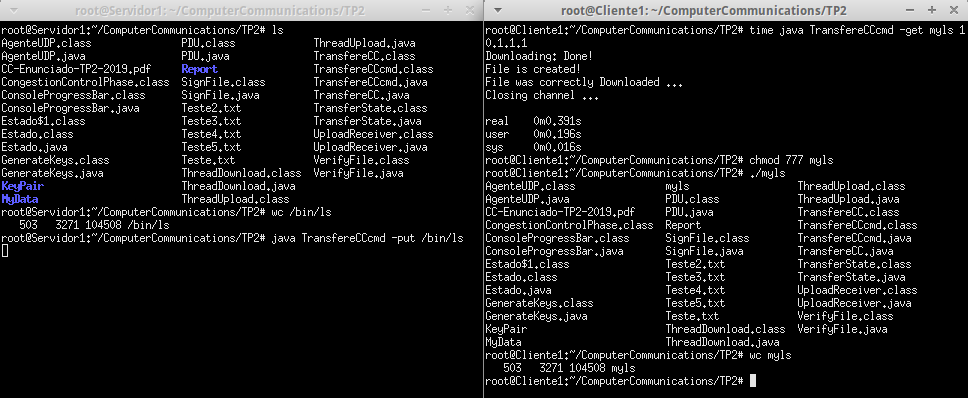
\includegraphics[scale=0.4]{myls_cliente1.png}
\end{center}
\caption{Transferência dum executável.}
\end{figure}

Agora, nesta imagem, é possível visualizar o Servidor1 a disponibilizar o executável, e o Alfa a realizar o download com sucesso. É importante referir que a ligação à LAN3, onde se encontra o Alfa, possui problemas na rede ao nível do congestionamento, e dessa forma, é previsível que existam algumas retransmissões. Tal é, de facto, possível reparar na seguinte imagem.

\begin{figure}[H]
\begin{center}
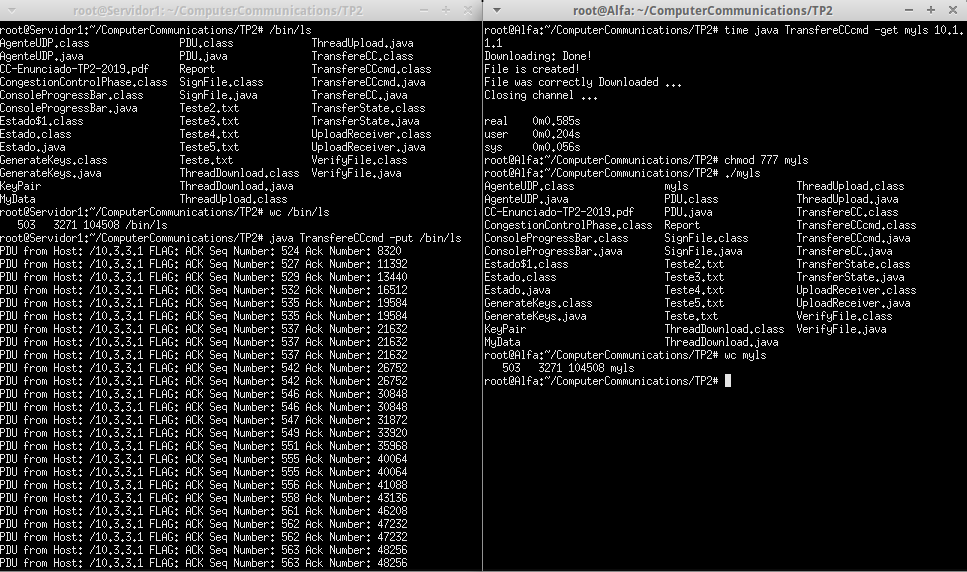
\includegraphics[scale=0.4]{myls_alfa.png}
\end{center}
\caption{Transferência dum executável para um recetor com congestionamento acentuado.}
\end{figure}



\section{Conclusões}



\end{document}
